\section{Result}
\label{sec:4_exp}

\subsection{Visualization} 

We developed a RShiny app for interactive visualization and exploratory data analysis in source-specific features. The app uses kmeans method to cluster sources using selected features. Also, the app utilizes Principal Component Analysis (PCA) analysis as a method to reduce dimension while retaining most significant information. Together, PCA1 and PCA2 provided another coordinate to analyze the effect of source grouping in a more visual-friendly way.

For RShiny part, the app uses multiple \texttt{observeEvent()} functions to update data grouping and the graph output in real-time. Details can be found in the source code provided.

\begin{figure}[ht]
    \centering
    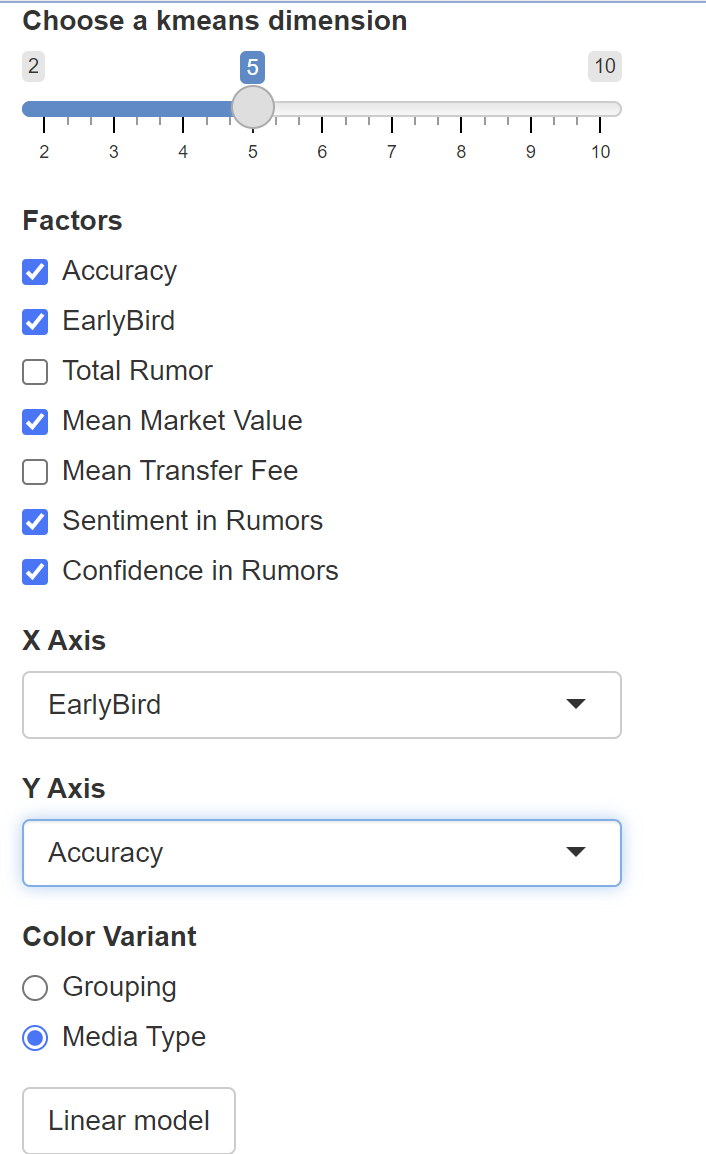
\includegraphics[width=.4\textwidth]{figs/shiny_ui.png}
    \caption{
        User interface of RShiny app
    }\label{fig:shiny_ui}
\end{figure}

As is shown in \autoref{fig:shiny_ui} from top to bottom, the user interface includes:
\begin{itemize}
    \item Dimension used for kmeans grouping
    \item Features used in kmeans grouping
    \item X axis: parameter used to draw the x axis (EarlyBird / Confidence / PCA1)
    \item Y axis: parameter used to draw the y axis (Accuracy / Sentiment / PCA2)
    \item Color variant: parameter used to color different rumor sources (kmeans Grouping / Media type)
    \item Linear model: adds a linear regression line to the chart
\end{itemize}

The output includes:
\begin{itemize}
    \item k-means Cluster Assignment Matrix: shows kmeans grouping result in each media type
    \item Scatter plot: Each point(or bubble) represents a rumor source we fetched. The size illustrates the quantity of rumors posted by the source. Colored by grouping, with legend.
\end{itemize}

The RShiny app can be utilized to discover more about the source-specific characteristics. Besides, to reveal more about properties of the sources we introduced a manually labelled \texttt{media type} label for each rumor source, which categorizes sources into five categories. They are:
\begin{itemize}
    \item \texttt{Club Specific Website}: Website dedicated to a specific club. Example: Liverpool, Chelsea, Arsenal
    \item \texttt{Mainstream Media}: Mainstream media that cover all sorts of news including football transfers. Example: BBC, The Guardian, The Telegraph 
    \item \texttt{Social Media}: Social media platforms with user generated content. Example: Facebook, X, Twitter
    \item \texttt{Sport Website}: Website dedicated to sports news only. Example: Skysports, 90 MIN
    \item \texttt{Other}: Source that can not be placed into categories above. Example: Youtube
\end{itemize}

The result we get as shown in \autoref{fig:shiny_result}, which suggests features of rumor source can be an indication of its actual media type. (e.g. club specific website have a long EarlyBird, as well as high confidence and accuracy, which may be explained by their inside news and long-term focus on surrounding a specific club; social media have a preference to cover transfer rumors of high-market-value football stars and have a high accuracy, which might be biased by confirmation posts; see more in detail in \autoref{tab:rumor_feature})

\begin{table}[htbp]
    \centering
    \caption{Features in each media type, mean value}
    \label{tab:rumor_feature}
    \begin{tabular}{lccccccc} % Make sure the number of 'c' matches the number of columns
        \toprule
        Rumor\_Label & accuracy & coverage & earlyBird & total\_rumor & marketvalue & fee & confidence \\
        \midrule
        Club Specific Website & 0.1909089 & \textit{0.01221372} & \textbf{121.33506} & \textit{29.00000} & \textit{13558507} & \textit{20085741} & \textbf{0.8503613} \\
        Social Media &\textbf{0.27028308} & 0.1127948 & \textit{45.32854} & 257.25000 & \textbf{25059916} & \textbf{31561311} & 0.6008637 \\
        Mainstream Media & 0.13433864 & \textbf{0.18828220} & 56.81000 & \textbf{271.03371} & 16448348 & 22086556 & 0.5833447 \\
        Sport Website &\textit{ 0.09570226} & 0.02412944 & 61.45449 & 67.09091 & 17020123 & 23037226 & \textit{0.5522350} \\
        Other & 0.15206255 & 0.03894491 & 60.56025 & 88.83333 & 21040859 & 26598533 & 0.5762029 \\
        \bottomrule
    \end{tabular}
\end{table}
\begin{figure}[ht]
    \centering
    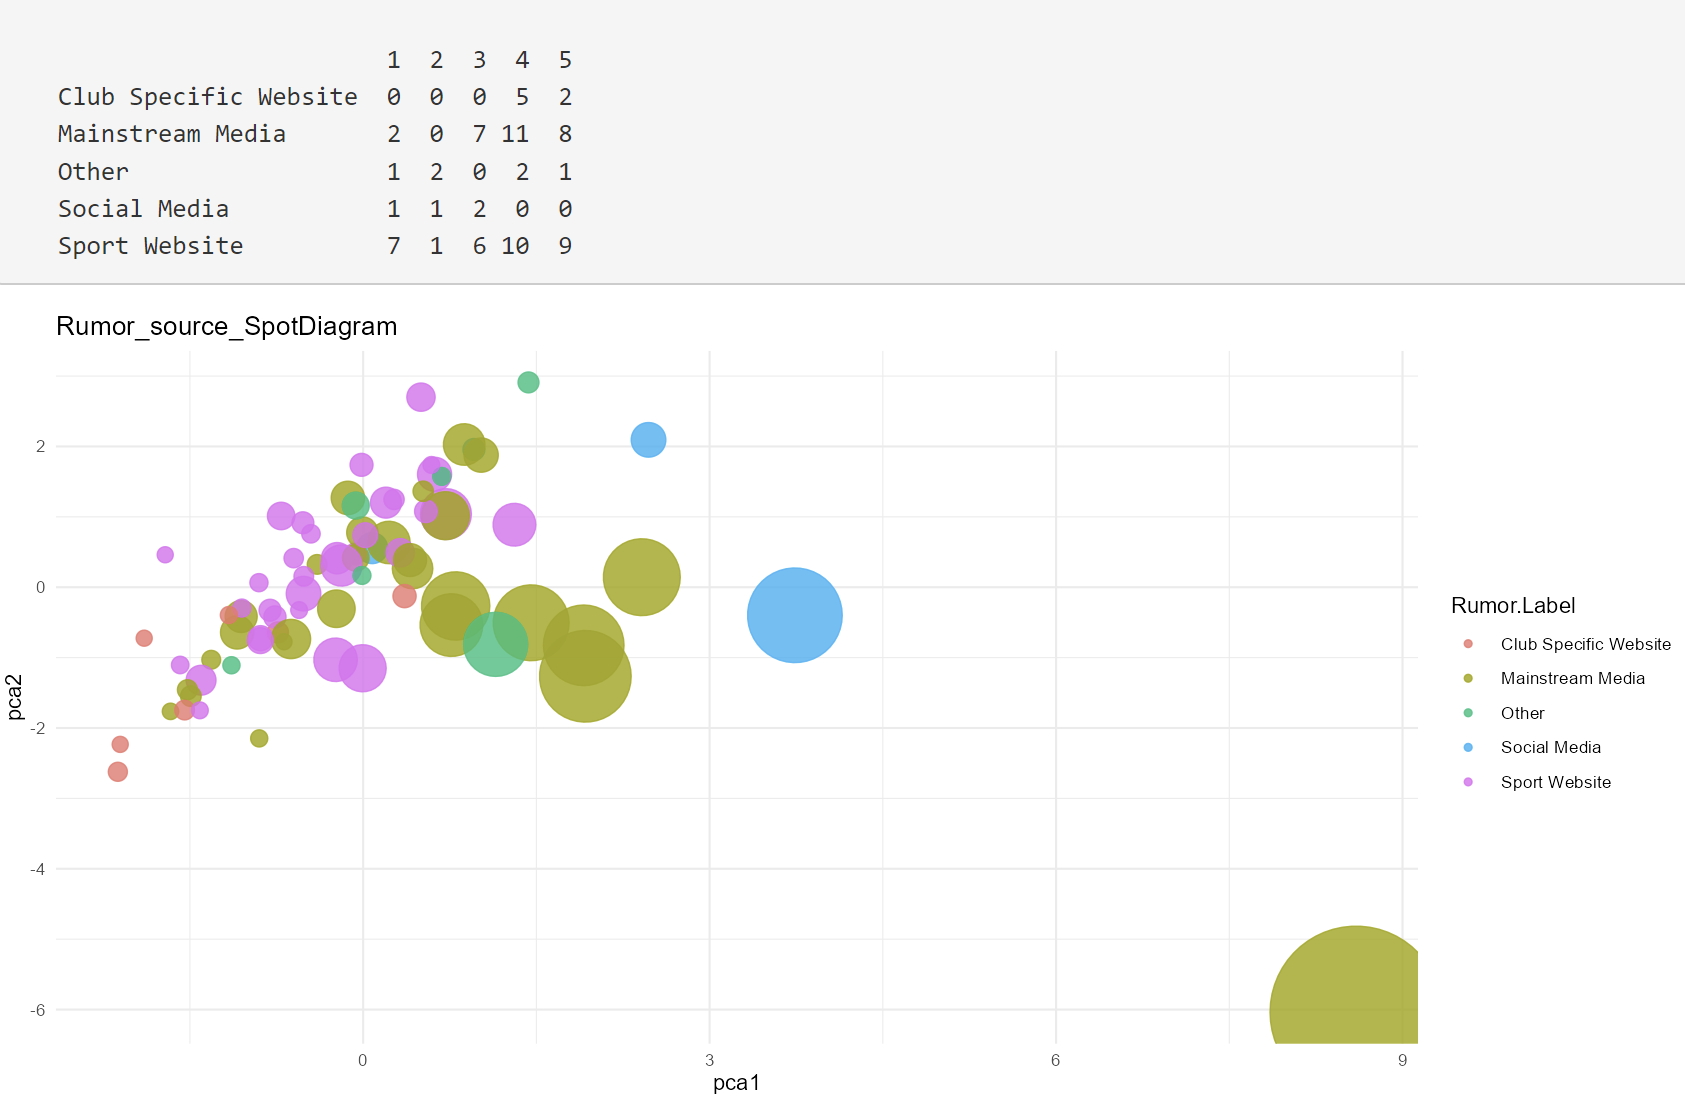
\includegraphics[width=.8\textwidth]{figs/shiny_result.png}
    \caption{
        k-means Cluster Assignment Matrix and Rumor Source Scatter plot
    }\label{fig:shiny_result}
\end{figure}

\subsection{Prediction}

\subsubsection{SVM}

Accuracy and 95\% CI:

\begin{itemize}
    \item \textbf{Accuracy:} 71.80\%
    \item \textbf{95\% CI:} (0.6919, 0.7431)
\end{itemize}

The following confusion matrix shows the performance of the Support Vector Machine (SVM) classifier:

\begin{table}[ht]
    \centering
    \begin{tabular}{|c|c|c|}
    \hline
    \textbf{Prediction / GT} & \textbf{FALSE} & \textbf{TRUE} \\
    \hline
    \textbf{FALSE} & \cellcolor{red!50} 429 & \cellcolor{cyan!50} 163 \\
    \hline
    \textbf{TRUE} & \cellcolor{cyan!60} 181 & \cellcolor{red!55} 447 \\
    \hline
    \end{tabular}
    \caption{Confusion Matrix for SVM}
    \label{tab:svm_cm}
\end{table}


\subsubsection{ElasticNet}

Accuracy and 95\% CI:

\begin{itemize}
    \item \textbf{Accuracy:} 73.61\%
    \item \textbf{95\% CI:} (0.7104, 0.7606)
\end{itemize}

ElasticNet performs better than the SVM model. The confusion matrix is shown as below:

\begin{table}[ht]
    \centering
    \begin{tabular}{|c|c|c|}
    \hline
    \textbf{Prediction / GT} & \textbf{FALSE} & \textbf{TRUE} \\
    \hline
    \textbf{FALSE} & \cellcolor{red!53} 438 & \cellcolor{cyan!45} 150 \\
    \hline
    \textbf{TRUE} & \cellcolor{cyan!55} 172 & \cellcolor{red!60} 460 \\
    \hline
    \end{tabular}
    \caption{Confusion Matrix for ElasticNet}
    \label{tab:elasticnet_cm}
\end{table}

\subsubsection{Random Forest}

Accuracy and 95\% CI:

\begin{itemize}
    \item \textbf{Accuracy:} 73.77\%
    \item \textbf{95\% CI:} (0.7121, 0.7622)
\end{itemize}

The Random Forest classifier achieved the highest accuracy of 73.77\%, a bit higher than ElasticNet. The confusion matrix for this model is as follows:

\begin{table}[ht]
    \centering
    \begin{tabular}{|c|c|c|}
    \hline
    \textbf{Prediction / GT} & \textbf{FALSE} & \textbf{TRUE} \\
    \hline
    \textbf{FALSE} & \cellcolor{red!65} 478 & \cellcolor{cyan!60} 188 \\
    \hline
    \textbf{TRUE} & \cellcolor{cyan!40} 132 & \cellcolor{red!50} 422 \\
    \hline
    \end{tabular}
    \caption{Confusion Matrix for Random Forest}
    \label{tab:rf_cm}
\end{table}

The feature importance in Random Forest was measured using the Gini index. The top 30 features with the highest Gini index are shown in the figure\ref{fig:rf_gini}.
     
\begin{figure}[ht]
    \centering
    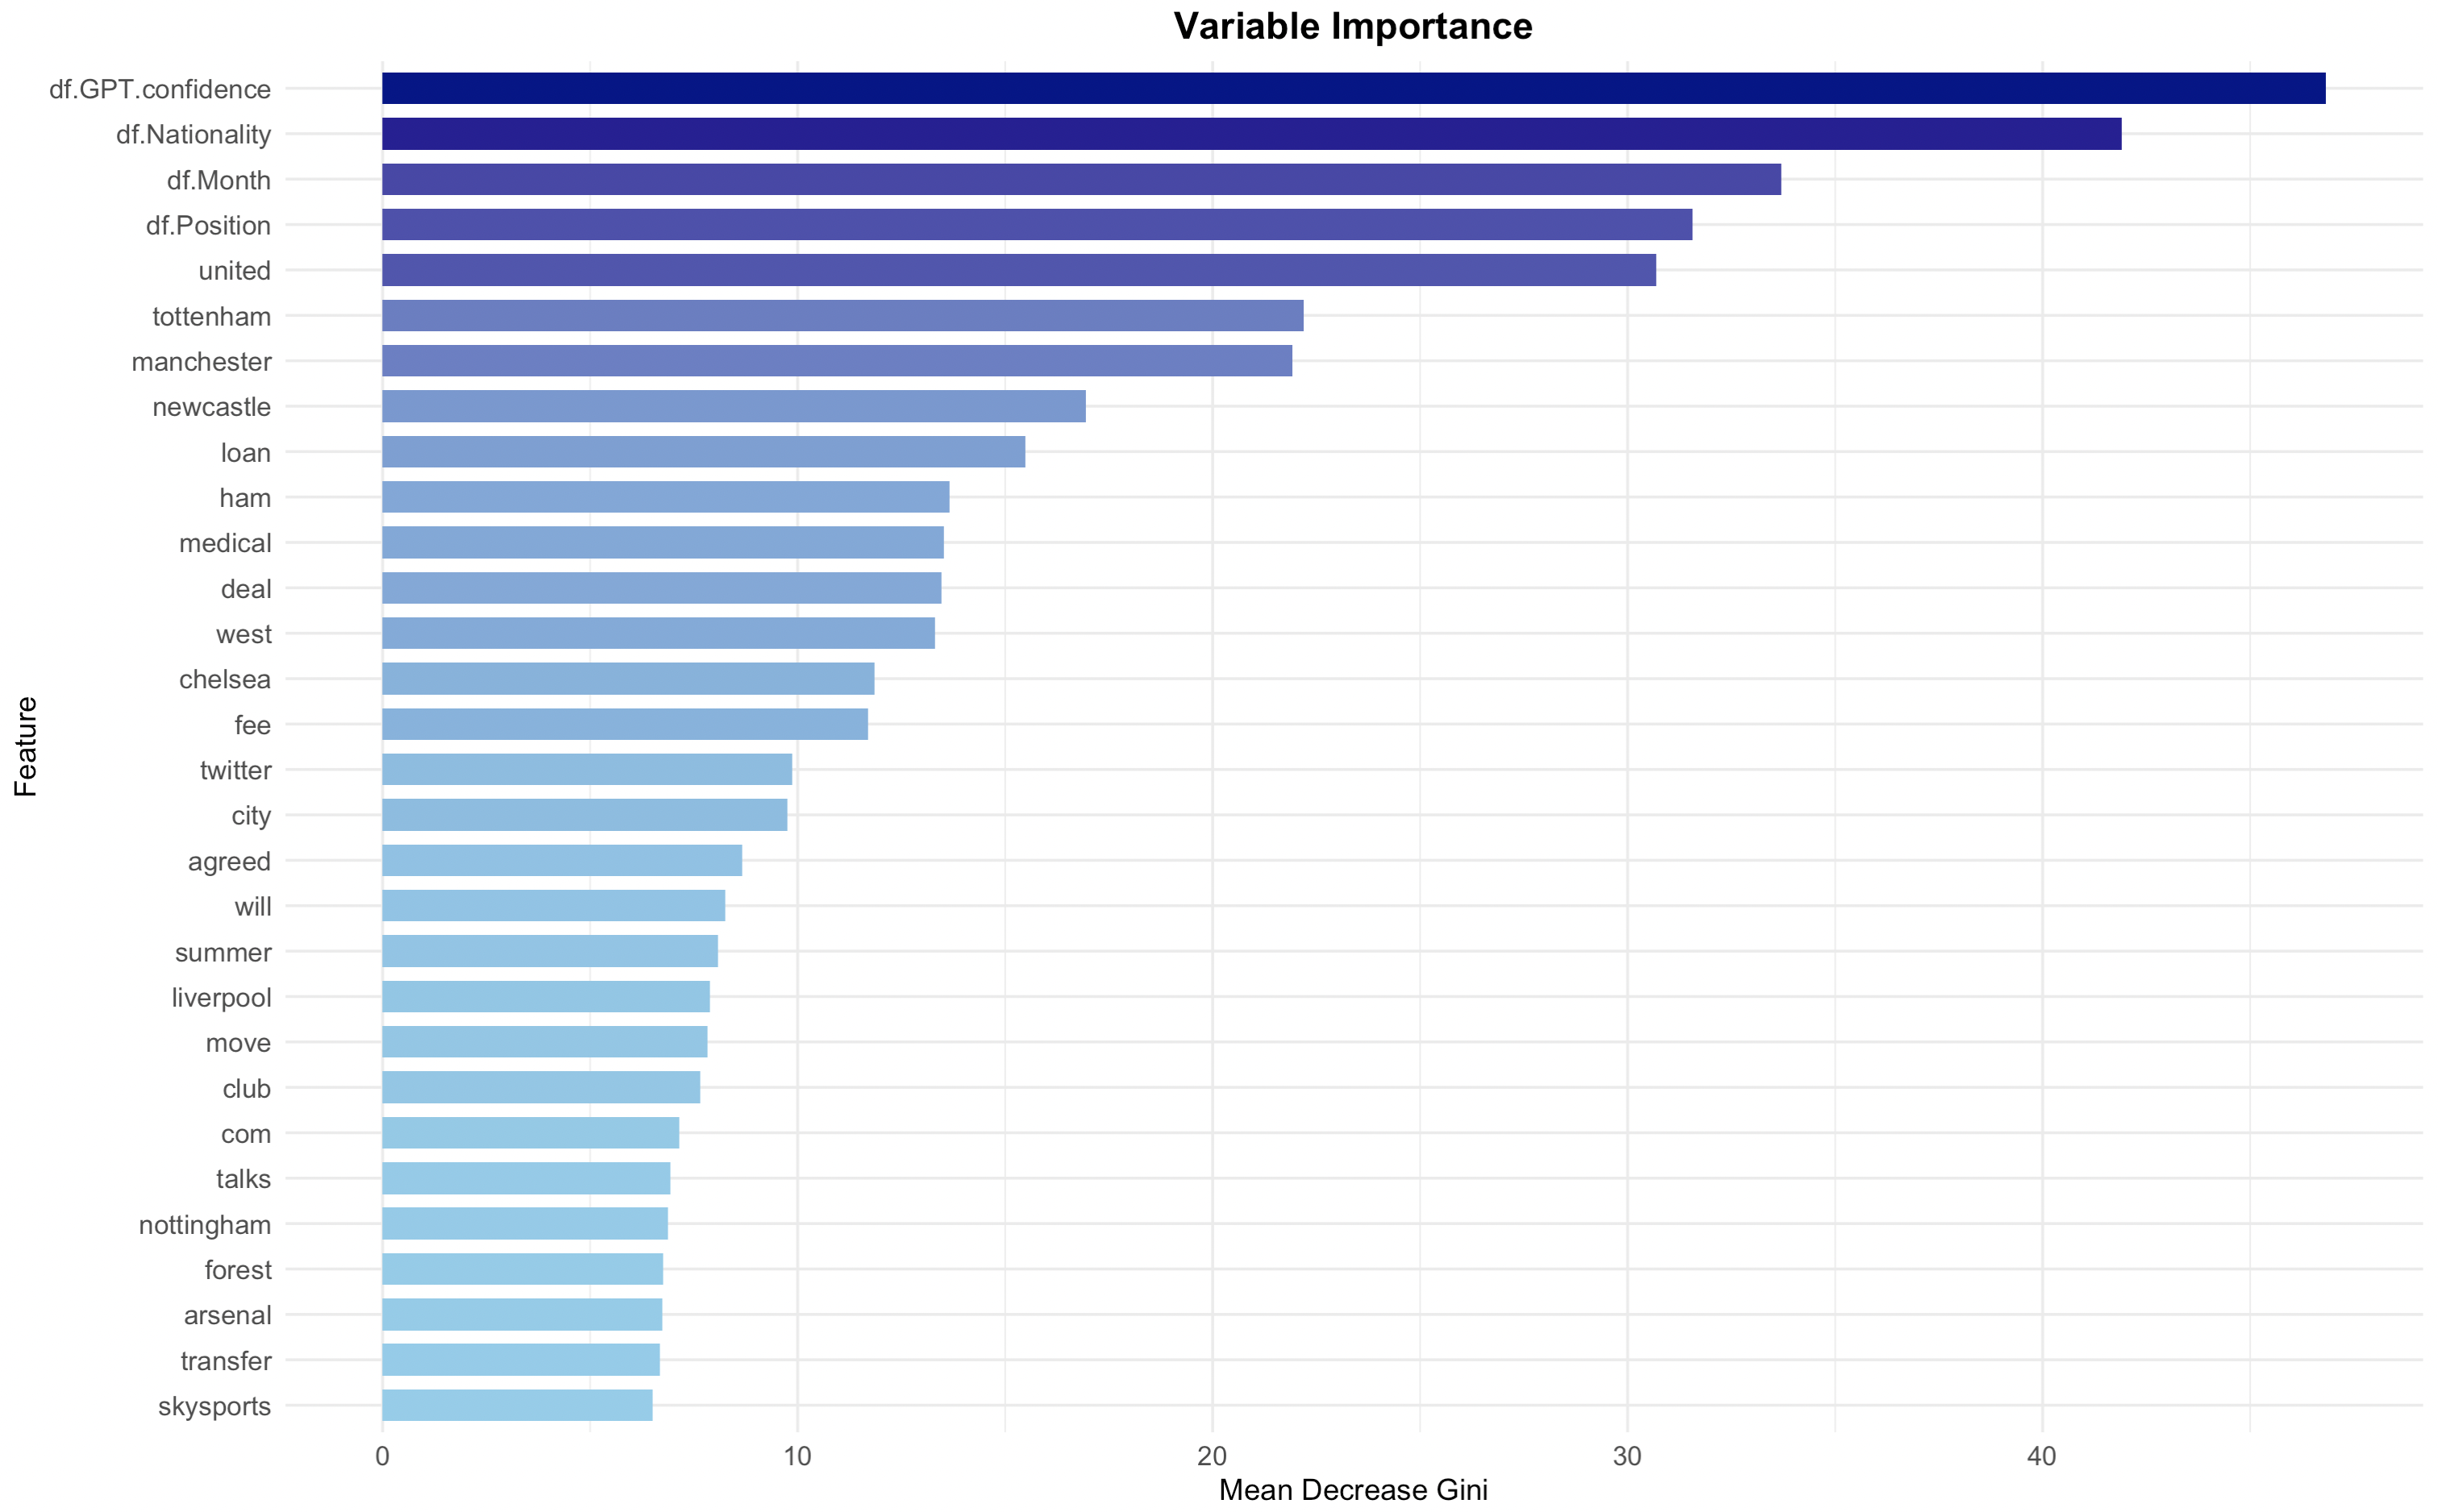
\includegraphics[width=.95\textwidth]{figs/rf_gini.png}
    \caption{Top 30 Features Based on Gini Index in Random Forest}
    \label{fig:rf_gini}
\end{figure}
